\documentclass[12pt,a4paper]{article}
\usepackage[portuguese]{babel}
\usepackage[a4paper]{geometry}
\usepackage[utf8]{inputenc}
\usepackage{lmodern}      % letra, símbolos, etc.
\usepackage{cmap}
\usepackage{setspace} % Espaçamento entre linhas 
\usepackage{microtype} % espaçamento entre letras e palavras, colocar depois da fonte
\usepackage{siunitx} % unidade si 
\sisetup{output-decimal-marker = {,}}
\usepackage[version=4]{mhchem}
\usepackage{caption} % caption
\usepackage{subcaption} % caption   
\usepackage{graphicx}     % gráficos
\usepackage{tabularx}     % tabelas
\usepackage{booktabs}  
\usepackage[table]{xcolor} % cores
\usepackage{multirow}
\usepackage{makeidx}
\usepackage{ragged2e}
\addto\captionsportuguese{\renewcommand{\refname}{Referências}}
\usepackage[colorlinks=true,citecolor=black,linkcolor=black,bookmarks=true]{hyperref}
\usepackage{natbib}
\usepackage{float}
\usepackage{indentfirst}

\onehalfspacing

\begin{document}

\pagenumbering{arabic}

\thispagestyle{empty}
\begin{minipage}{\textwidth}\centering
Universidade de São Paulo \\
Instituto de Ciências Matemáticas e Computação \\
Desenvolvimento de Código Otimizado - SSC 0951 \\
\end{minipage}

\vspace{5cm}

\begin{minipage}{\textwidth}\centering
\Large Relatório Trabalho 1  \\
\vspace{2cm}
\Large \textbf{Profilling: Loop Interchange e Loop Unrolling}
\end{minipage}

\vspace{3cm}

\begin{minipage}{\linewidth}\centering
\begin{enumerate}
     \item Lucas G. Meneses   \space \space \space \space \space \space  Número: 13671615
      \item Henrique S. Marques  \space \space Número: 11815722
      \item Carlos F. C. Lemos  \space \space \space \space Número: 12542630
      \item Eduardo S. Rocha  \space \space \space \space \space \space Número: 11218692
\end{enumerate}
\end{minipage}

\vfill

\begin{minipage}{\linewidth}
\centering\today, \\
São Carlos, SP, \\
Brasil
\end{minipage}

\clearpage
\thispagestyle{empty}

\tableofcontents

\section{Introdução}

A atividade 1 da disciplina "Desenvolvimento de Código Otimizado"{~} teve como objetivo introduzir conceitos relacionados à \textit{Profilling} utilizando a ferramenta \href{https://perf.wiki.kernel.org}{perf}, bem como a análises estatísticas referentes a desempenho de código e duas técnicas de otimização de laços: \textit{loop interchange} e \textit{loop unrolling}, em cenários com alocação estática (AE) e dinâmica (AD).

O \textit{perf} é uma ferramenta que se destaca por sua capacidade de aproveitar os contadores de desempenho disponíveis em CPUs modernas para realizar análises detalhadas do desempenho de aplicações. Permite que administradores e desenvolvedores coletem dados referentes a eventos de hardware e software, bem como tempos de execução de funções. Uma das aplicações mais notáveis do \textit{perf} é o \textit{profilling} de aplicações, permitindo a identificação de gargalos de desempenho, ineficiências de código e otimizações críticas. Através da captura precisa de eventos de desempenho, como ciclos de CPU, \textit{branch predictions} e cache \textit{misses}, o \textit{perf} oferece uma visão profunda do comportamento do sistema, facilitando a melhoria da eficiência e a resolução de problemas de desempenho.

Quanto às técnicas de otimização de laços, o \textit{loop interchange} e \textit{loop unrolling} são amplamente utilizadas em programação para melhorar o desempenho de código. O \textit{loop interchange} envolve a reorganização das iterações de um \textit{loop}, muitas vezes para melhorar o acesso à memória e maximizar a eficiência da cache. Isso pode reduzir os tempos de espera por dados e melhorar significativamente o desempenho. Por outro lado, o \textit{loop unrolling} busca diminuir a sobrecarga de um \textit{loop}, onde várias iterações são combinadas em uma única iteração maior. Isso pode reduzir instruções de controle do \textit{loop} e melhorar o paralelismo, tornando o código mais eficiente. Ambas as técnicas são valiosas para otimizar laços em programas, adaptando-se a diferentes cenários e requisitos de desempenho.

\section{Metodologia}

Para a realização de todos os experimentos, foi utilizado um computador rodando o Sistema Operacional Ubuntu, cuja CPU é um Intel Core i5 6600k com frequência de \textit{clock} de \SI{3,5}{\giga\hertz}, 4 núcleos e 4 \textit{threads}. Quanto à memória, o computador faz uso de \SI{16}{\giga\byte} de RAM do tipo DDR4, cache L1 de dados e de instruções ambas 8-\textit{way} com $4 \times \SI{32}{\kilo\byte}$ de capacidade, L2 4-\textit{way} $4 \times \SI{256}{\kilo\byte}$ e L3 12-\textit{way} de \SI{6}{\mega\byte}. 

Ademais, 6 seções de experimentos foram realizadas, todas utilizando multiplicação de matrizes quadradas de tamanho $800$:

\begin{itemize}
    \item Sem otimização, utilizando AE
    \item Sem otimização, utilizando AD
    \item Com \textit{loop interchange}, utilizando AE
    \item Com \textit{loop interchange}, utilizando AD
    \item Com \textit{loop unrolling}, utilizando AE
    \item Com \textit{loop unrolling}, utilizando AD
\end{itemize}

Em todas as seções, o código foi executado 10 vezes utilizando \textit{perf} e as métricas observadas foram: (i) tempo de resposta; (ii) quantidade absoluta de cache \textit{loads}; (iii) quantidade absoluta de cache \textit{misses}; (iv) quantidade absoluta de instruções tipo \textit{branch}; (v) quantidade absoluta de \textit{branch-misses}.  Dessa forma, a análise dos resultados (Seção \ref{sec:resultados}) obtidos foi subdivida em duas partes distintas, a primeira destinada apenas aos tempos de resposta (Seção \ref{sec:resultados_tempo}) e outra à análise de influência de fatores (Seção \ref{sec:resultados_fatores}). 

Para verificação dos tempos de resposta, as médias aritméticas das 10 amostras de cada seção foram calculadas juntamente de seus invervalos de confiança (\SI{95}{\percent}) para efeitos de comparação. Quanto à influência de fatores, todos os cálculos foram realizados, bem como os \textit{plots} gerados, utilizando o \textit{script} em $R$ fornecido via e-Disciplinas. 

\section{Resultados} \label{sec:resultados}

\subsection{Tempos de Resposta} \label{sec:resultados_tempo}

Como pode ser observado na Figura \ref{fig:tempo_resposta}, a técnica de otimização \textit{loop interchange} foi a que levou aos melhores resultados em relação ao tempo de resposta (tempo total de execução do programa), tanto com AD quanto com AE, sendo aproximadamente meio segundo mais rápido que a execução sem otimização com AE, a terceira com melhor desempenho. Neste caso, o tipo de alocação não trouxe mudanças significativas no tempo e, também, os valores permaneceram similares ao longo das 10 amostragens, fenômeno observado pelos intervalos de confiança pequenos. 

Diferentemente do \textit{loop interchange}, o \textit{loop unrolling} apresentou diferenças significativas ao se alterar o método de alocação, tendo melhor desempenho com AE. O mesmo pôde ser observado quando nenhuma técnica de otimização foi aplicada. Nesse sentido, a melhora de desempenho da AE em comparação à AD é explicada pela melhor localidade espacial da AE, tendo em vista que o endereçamento é conhecido em tempo de compilação e, assim, há vantagens quanto ao aproveitamento da cache. Esta observação foi confirmada através da análise de influência de fatores discutida na Seção \ref{sec:resultados_fatores}.

Ademais, a Figura \ref{fig:tempo_resposta} também indica que a técnica \textit{loop unrolling} não trouxe mudanças relevantes nos tempos de resposta, em especial pela equivalência com o desempenho dos experimentos sem técnicas de otimização (claro, quando utilizado o mesmo modo de alocação), tendo em conta os intervalos de confiança sobrepostos. 

\begin{figure}[H]
\centering
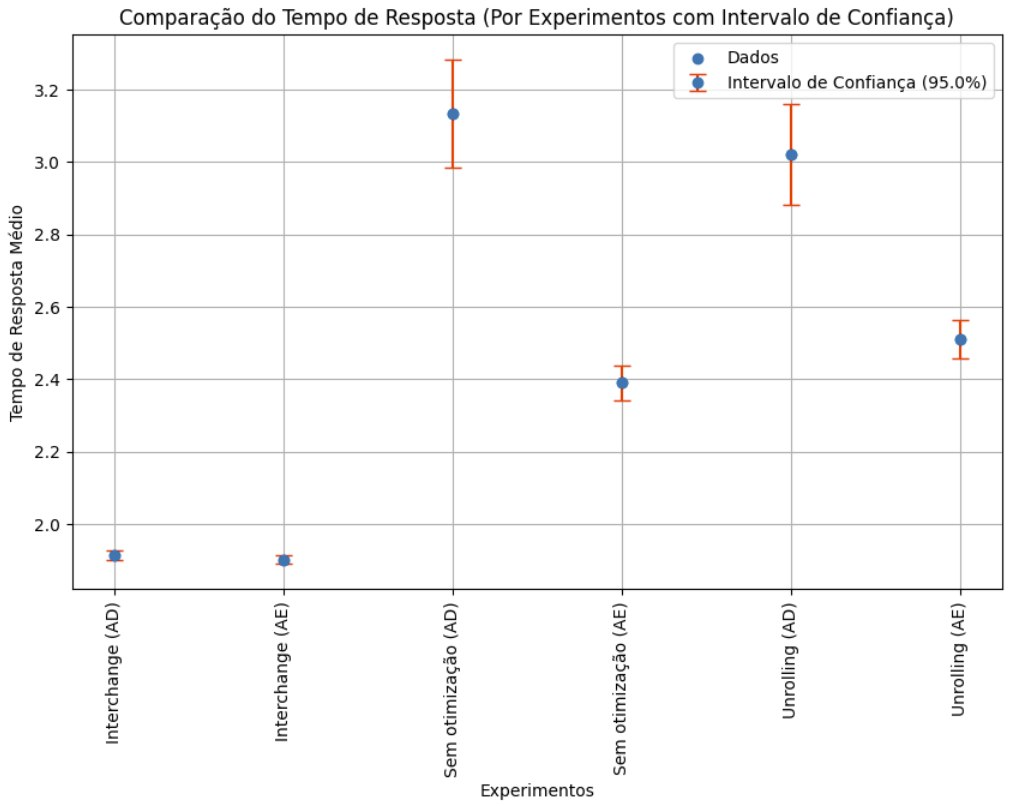
\includegraphics[width=0.90\linewidth]{Figures/fig_tempo_resposta.jpg}
\caption{Tempos de resposta (\si{\second}) em função do experimento realizado. Os círculos azuis indicam a média dos dados obtidos para cada experimento e as barras vermelhas mostram o intervalo de confiança de \SI{95}{\percent}.}
\label{fig:tempo_resposta}
\end{figure}

\subsection{Análise de Influência de Fatores} \label{sec:resultados_fatores}

Como pode ser visto pela Figura \ref{fig:influencia_fatores}, a influência da técnica de otimização e do método de alocação varia de acordo com o parâmetro utilizado como referência. Nesse sentido, os gráficos podem ser facilmente interpretados ao avaliar a posição relativa entre os pontos: quanto mais similares as alturas, menos alterações a técnica de otimização ou de alocação causam no parâmetro observado.  


Pelo Gráfico \ref{sub_fig:cache_loads}, vemos que não há diferenças significativas no número absoluto de cache \textit{loads} quando o \textit{loop interchange} é utilizado ou não. Entretanto, a AE apresentou um menor número de cache \textit{loads}, por motivos previamente discutidos na Seção \ref{sec:resultados_tempo}. Já em relação ao número absoluto de cache \textit{misses} (Figura \ref{sub_fig:cache_misses}), o uso do \textit{loop interchange} foi responsável por diminuí-lo, enquanto a técnica de alocação pouco influenciou. Este resultado pode explicar, majoritariamente, o motivo pelo qual esta técnica de otimização obteve os melhores tempos de resposta.


Em relação às \textit{branches}, o número absoluto de instruções deste tipo diminuiu consideravelmente com o uso do \textit{loop unrolling}, fenômeno completamente esperado tendo em vista o principal objetivo da técnica: diminuir a quantidade de iterações e, consequentemente, a quantidade de \textit{branches}. Por outro lado, a quantidade de \textit{branch misses} permaneceu constante mesmo com a utilização do \textit{unrolling}, o que pode explicar, em partes, o porquê desta técnica não ter melhorado o desempenho do código de maneira significativa. Por fim, o modo de alocação foi influente no número de \textit{branch misses} (cerca de $3000$ \textit{branch misses} a mais, em média, com uso de AD). 

\begin{figure}[H]
\centering

\begin{subfigure}{0.49\linewidth}
    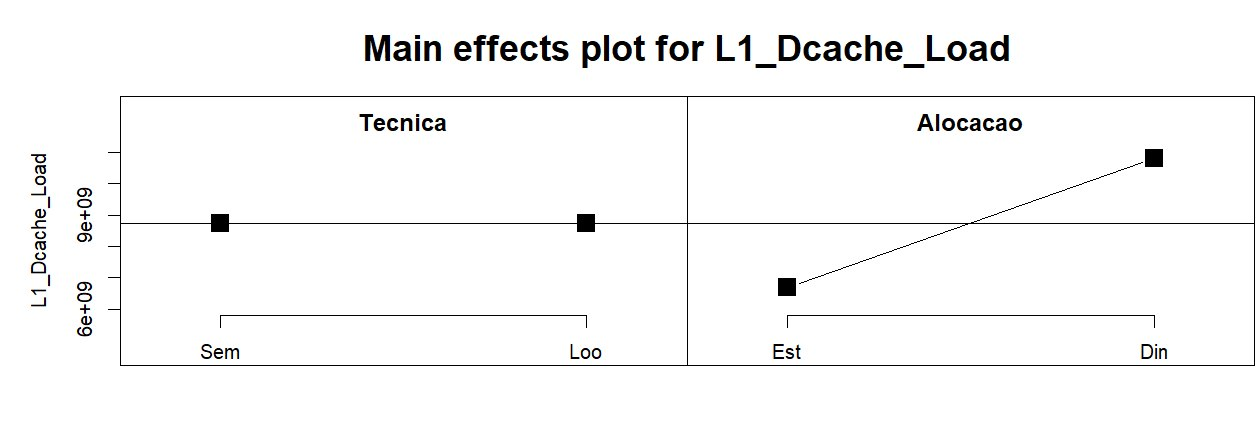
\includegraphics[width=\linewidth]{Figures/fig_fatores_cache_load.jpg}
    \caption{Influência do fator cache \textit{load} (\textit{loop interchange}).}
    \label{sub_fig:cache_loads}
\end{subfigure}
\hfill
\begin{subfigure}{0.49\linewidth}
    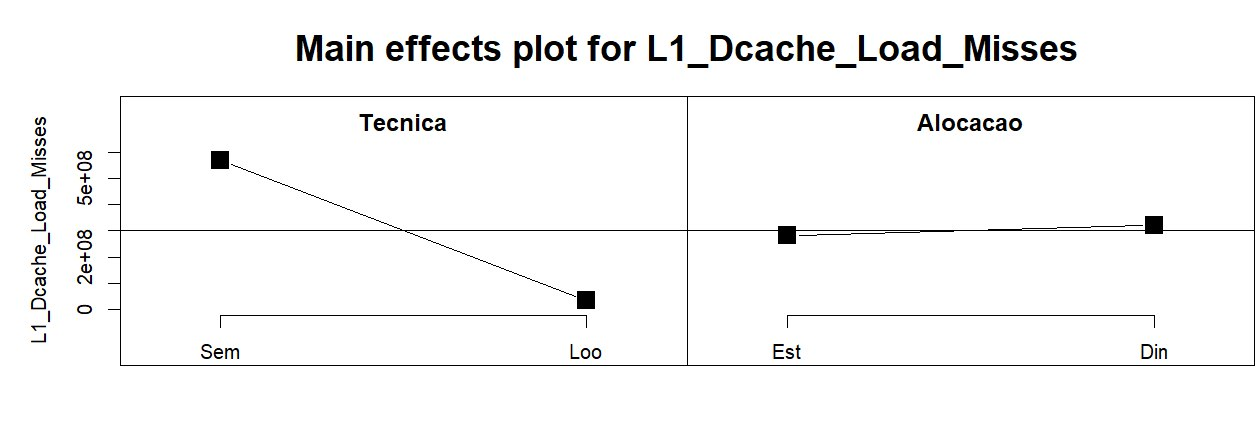
\includegraphics[width=\linewidth]{Figures/fig_fatores_cache_misses.jpg}
    \caption{Influência do fator cache \textit{misses} (\textit{loop interchange}).}
    \label{sub_fig:cache_misses}
\end{subfigure}

\begin{subfigure}{0.49\linewidth}
    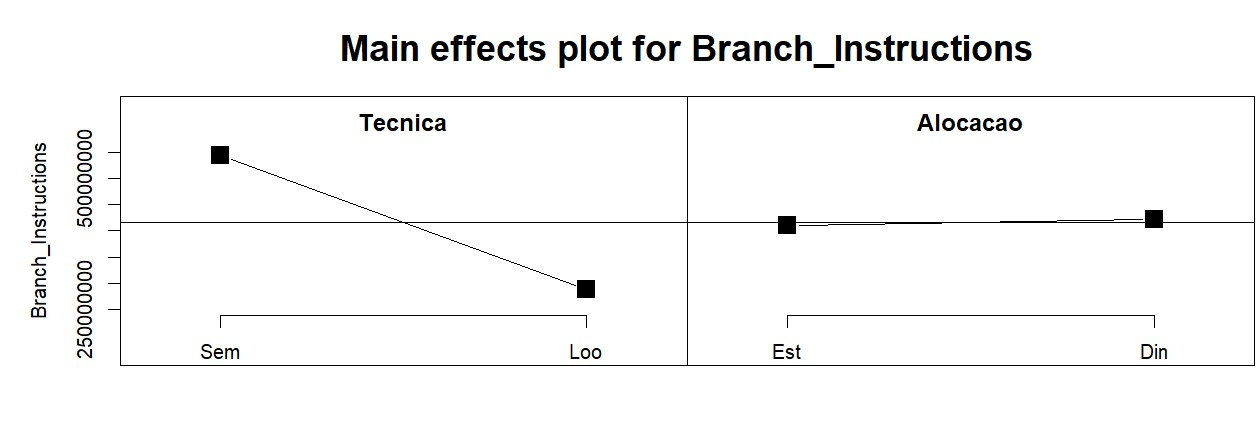
\includegraphics[width=\linewidth]{Figures/fig_fatores_instrucoes_branch.jpg}
    \caption{Influência do fator instruções \textit{branch} (\textit{loop unrolling}).}
    \label{sub_fig:instrucoes_branch}
\end{subfigure}
\hfill
\begin{subfigure}{0.49\linewidth}
    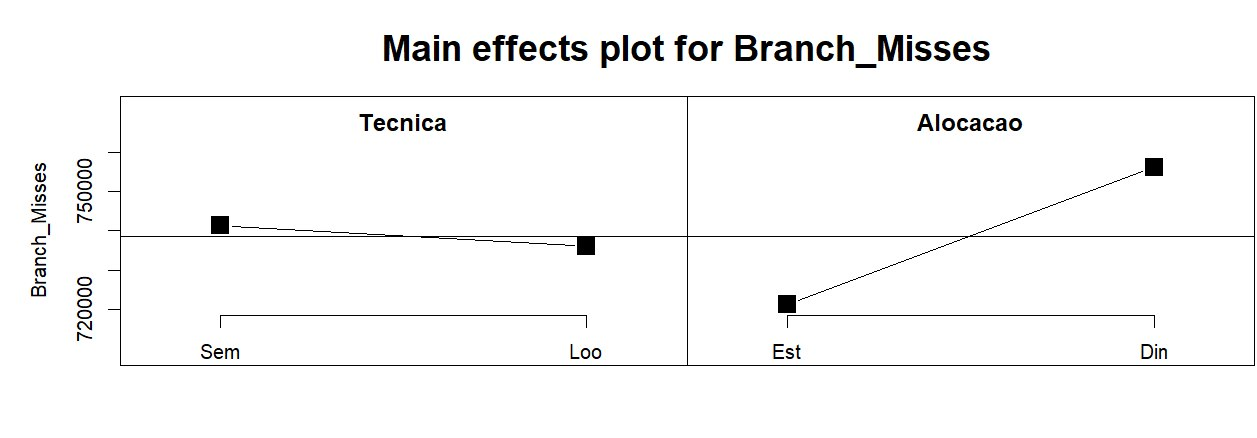
\includegraphics[width=\linewidth]{Figures/fig_fatores_branch_misses.jpg}
    \caption{Influência do fator \textit{branch misses} (\textit{loop unrolling}).}
    \label{sub_fig:branch_misses}
\end{subfigure}

\caption{Análise de Influência de Fatores. Em cada figura da matriz, avaliamos se a técnica de otimização e/ou o modo de alocação interferiram nos fatores avaliados pelo estudo.}
\label{fig:influencia_fatores}
\end{figure}

\section{Conclusões} \label{sec:conclusoes}

Neste estudo, investigamos o desempenho de técnicas de otimização de código, especificamente \textit{loop interchange} e \textit{loop unrolling}, em conjunto de diferentes métodos de alocação de memória, no contexto de tempo de resposta e de outros marcadores de desempenho. Os resultados obtidos proporcionam alguns \textit{insights} sobre o impacto dessas técnicas em vários aspectos.

A técnica de otimização \textit{loop interchange} demonstrou ser altamente eficaz na melhoria do tempo de resposta do programa. Através da reorganização das estruturas de \textit{loops}, conseguimos reduzir significativamente o tempo total de execução em relação à execução sem otimização, obtendo uma economia de aproximadamente meio segundo. Além disso, a alocação de memória, seja dinâmica (AD) ou estática (AE), não exerceu uma influência significativa no desempenho quando esta técnica foi aplicada, como evidenciado pela similaridade dos resultados ao longo das 10 amostragens. Além disso, a análise de influência de fatores revelou que o \textit{loop interchange} teve um impacto positivo no número absoluto de cache \textit{misses}, contribuindo para a melhoria do tempo de resposta. 

Em contraste, o \textit{loop unrolling} apresentou um impacto menos pronunciado no tempo de resposta do programa. Embora tenha reduzido significativamente o número absoluto de instruções \textit{branch}, não conseguiu melhorar substancialmente o desempenho geral. O número de \textit{branch misses} permaneceu praticamente inalterado, independentemente de ser aplicada ou não esta técnica.

Em resumo, este estudo ressalta a importância de escolher as técnicas de otimização apropriadas para um determinado contexto e considerar cuidadosamente o impacto do método de alocação de memória. Para programas sensíveis ao desempenho, a aplicação de técnicas como o \textit{loop interchange} pode resultar em melhorias notáveis nos tempos de resposta, enquanto o \textit{loop unrolling} pode ser mais adequado quando a redução no número absoluto de instruções \textit{branch} é de suma importância.

\end{document}